\documentclass{DIKU-article}[2006/05/09]
\usepackage[utf8]{inputenc}

%% Skabelon til LiCS-afleveringer

%%%%%%%%%%%%%%%%%%%%%%%%%%%%%%%%%%%%%%%%%%%%%%%%%%%%%%%%%%%%%%%
%% Begynd preamble
%%%%%%%%%%%%%%%%%%%%%%%%%%%%%%%%%%%%%%%%%%%%%%%%%%%%%%%%%%%%%%%

%% Til at tegne træer!
\usepackage{tikz}
%% Til at kunne have billeder
\usepackage{graphicx}
%% Til at kunne have source code
\usepackage{listings}
\lstset{
  breaklines=true,
  keepspaces=true,
  frame=ltrb,
  framesep=1pt,
  commentstyle=\color{Brown},
  basicstyle=\ttfamily\footnotesize,
  numbers=left,
  title=\lstname,
  columns=fullflexible,
  extendedchars=\true,
  inputencoding=ansinew,
}

%% Font and input encoding
%% Tillad æøå
\usepackage[T1]{fontenc}
%% Babel (language)
%\usepackage[UKenglish]{babel} % If you write in English
\usepackage[UKenglish]{isodate}
%\usepackage{parskip}
\usepackage{booktabs}
%\usepackage[danish]{babel} % Hvis du skriver på dansk

%% Til links
\usepackage{hyperref}

%% AMS-Math packages
%\usepackage{amsmath}
%\usepackage{amssymb}
%\usepackage{amsthm}
%% Extra symbols that we almost always need
%\usepackage{stmaryrd}
\usepackage{color}
\usepackage{url}
\usepackage{semantic}
\usepackage{fancyref}
\usepackage{enumitem}


% Figure subcaptions
\usepackage{subcaption}

% forkortelse af texttt!
\newcommand{\tbf}{\textbf}
\newcommand{\ttt}{\texttt}
\newcommand{\tit}{\textit}

% Sorting networks
% Credit to whoever wrote this for the 'Applying Sorting Networks to Synthesize
% Optimized Sorting Libraries' M. Codish, L. Cruz-Filipe, M. Nebel, P.
% Schneider-Kamp (https://arxiv.org/abs/1505.01962)
\usepackage[trim]{tokenizer}
\newcounter{sncolumncounter}
\newcounter{snrowcounter}

\def \nodelabel#1{%
\setcounter{snrowcounter}{1}
 \foreach \i in {#1}{%
   \draw (\sncolwidth*\value{sncolumncounter},\value{snrowcounter}) node[anchor=south]{\i};
   \addtocounter{snrowcounter}{1}
 }
\addtocounter{snrowcounter}{-1}
 \addtocounter{sncolumncounter}{1}
}

\newcommand{\sncolwidth}{0.7} %

\def \addcomparator#1#2{%
    \draw (\sncolwidth*\value{sncolumncounter},#1) node[circle,fill=black,minimum size=4pt,inner sep=0pt,outer sep=0pt]{}--(\sncolwidth*\value{sncolumncounter},#2) node[circle,fill=black,minimum size=4pt,inner sep=0pt,outer sep=0pt]{};
}

\newcommand{\addrevcomparator}[3][0.5]{
    \draw[>=stealth,postaction={decorate},decoration={markings,mark=at position #1 with {\arrow[scale=2]{<}}}] (\sncolwidth*\value{sncolumncounter},#2) node[circle,fill=black,minimum size=4pt,inner sep=0pt,outer sep=0pt]{}--(\sncolwidth*\value{sncolumncounter},#3) node[circle,fill=black,minimum size=4pt,inner sep=0pt,outer sep=0pt]{};
}

\def \addhalfcomparator#1#2{%
    \draw (\sncolwidth*\value{sncolumncounter},#1) node[circle,fill=black,minimum size=4pt,inner sep=0pt,outer sep=0pt]{}--(\sncolwidth*\value{sncolumncounter},#2);
}

\def \addlayer{%
  \addtocounter{sncolumncounter}{1}
}

\def \nextlayer{%
  \draw [dashed] (\sncolwidth*\value{sncolumncounter}+\sncolwidth,0.6)--(\sncolwidth*\value{sncolumncounter}+\sncolwidth,\value{snrowcounter}+0.6);
  \addtocounter{sncolumncounter}{2}
}

\newcommand{\addarrow}[5][0.75]{
  \draw[>=stealth,postaction={decorate},line width=1.5 pt,decoration={markings,mark=at position #1 with {\arrow[scale=1.2]{>}}}] (\sncolwidth*#2,#3)--(\sncolwidth*#4,#5);
}
\def \nodeconnection#1{%
  \foreach \i in {#1}{%
    \GetTokens{nodesrc}{nodedest}{\i}
    \draw (\value{sncolumncounter}*0.7,\nodesrc) node[circle,inner sep=0pt,minimum size=3pt,fill=black]{}--(\value{sncolumncounter}*0.7,\nodedest) node[circle,inner sep=0pt,minimum size=3pt,fill=black]{};
  }
  \addtocounter{sncolumncounter}{1}
}
\newenvironment{sortingnetwork}[2]
{
  \setcounter{sncolumncounter}{0}
  \setcounter{snrowcounter}{#1}
  \def \sn@fullsize{15}
  \begin{tikzpicture}[scale=#2*0.7]
}
{
  \foreach \i in {1, ..., \value{snrowcounter}}
  {
    \draw (-\sncolwidth,\i)--(\sncolwidth*\value{sncolumncounter}+\sncolwidth,\i);
  }
  \end{tikzpicture}
}
% End sorting networks



%%%%%%%%%%%%%%%%%%%%%%%%%%%%%%%%%%%%%%%%%%%%%%%%%%%%%%%%%%%%%%%
%% Slut preamble -- herunder følger selve dokumentet!
%%%%%%%%%%%%%%%%%%%%%%%%%%%%%%%%%%%%%%%%%%%%%%%%%%%%%%%%%%%%%%%

\titlehead{Algorithm Engineering - Project}
\authorhead{C. Johnsen, M. Poulsen and D. Pedersen}
\title{Algorithm Engineering}
\author{Carl-Johannes Johnsen (grc431) \and Martin Philip Poulsen (jfw772) \and Daniel Lundberg
Pedersen (vzb687)}

\institute{%
    Department of Computer Science, University of Copenhagen\\
    Universistetsparken 5, DK-2100 Copenhagen East, Denmark\\
    \email{\{grc431,jfw772,vzb687\}@alumni.ku.dk}%
}

\dates{2016-10-30}


\begin{document}
\maketitle

\section{Parallel}
In this section, we will be looking at parallelising sorting algorithms. We
will be looking at sorting elements residing within the \texttt{vector} data
structure. Since we are trying to shave off time, we start by looking into
different approaches to memory management, allocation and access. From there we
will be implementing sequential versions of Quicksort and Mergesort. Then we
will be parallelising these algorithms, and finally combine a combination of
both.

\subsection{Approaches to pivot choosing, memory allocation, management and
access}
Here we will be looking at choosing a good pivot, inserting elements into a new
empty \texttt{vector}, moving data from one \texttt{vector} to another, moving
data from one \texttt{vector} into an empty one and extracting a subset
\texttt{vector} from a \texttt{vector}.

\subsubsection{Choosing the right pivot}
We have three approaches: choosing a random element, choosing the middle
element and choosing the median of three random elements. The goal is to choose
a pivot element, which will as much as possible split the input into equal
subsets.

It has been showed that choosing a random element is usually good in practice.
However, getting a random number can introduce some overhead, which is why we
also tried the middle element approach. We could also have chosen to just
selecting the first or the last element, however, this would be bad in the case
of sorted or reversed sorted input. Finally, we tried the median of three
approach, as the chances of choosing three elements, which are all bad, is less
than the probability for making a single bad choice.

First, we look at how good the splits are:
\begin{center}
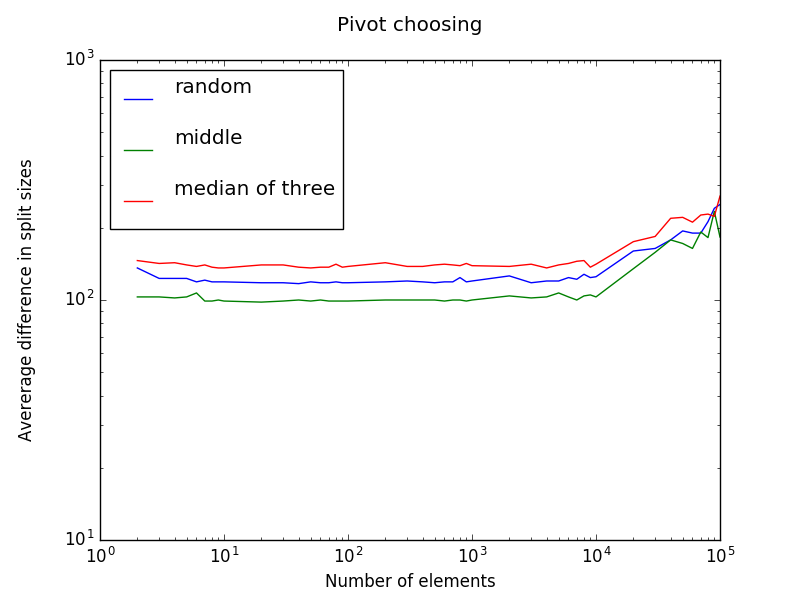
\includegraphics[width=.5\linewidth]{graphs/pivot_split}
\end{center}
Interestingly enough, choosing the middle element as pivot works suprisingly
well on random input.

Then, we look at the perfomance of the three:
\begin{center}
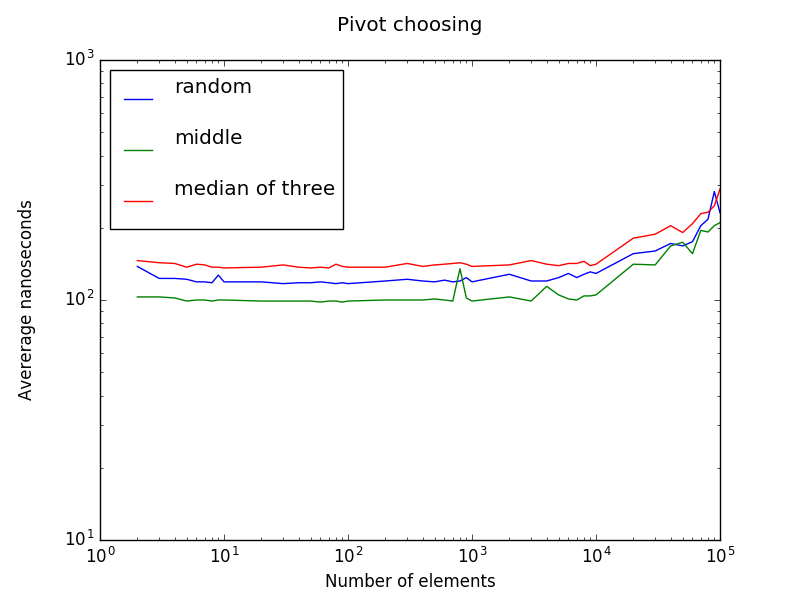
\includegraphics[width=.5\linewidth]{graphs/pivot_perf}
\end{center}
Here, we see that the median of three performs the worst. This was expected, as
it requires more work. Coming in second is the random element, as the
beforementioned overhead from getting random numbers is present. Finally, we
have the best performance from choosing the middle element, which again is
expected as it has the least work to do.

\subsubsection{Memory allocation}
Within the different algorithms, we sometimes want to insert one element at a
time into a \texttt{vector}. We have two approaches: calling \texttt{vector.insert()}
one element at a time, and calling \texttt{vector.push\_back()}. For each we look at
the performance with and without calling \texttt{vector.reserve()}.

We have \texttt{vector.insert()}:
\begin{center}
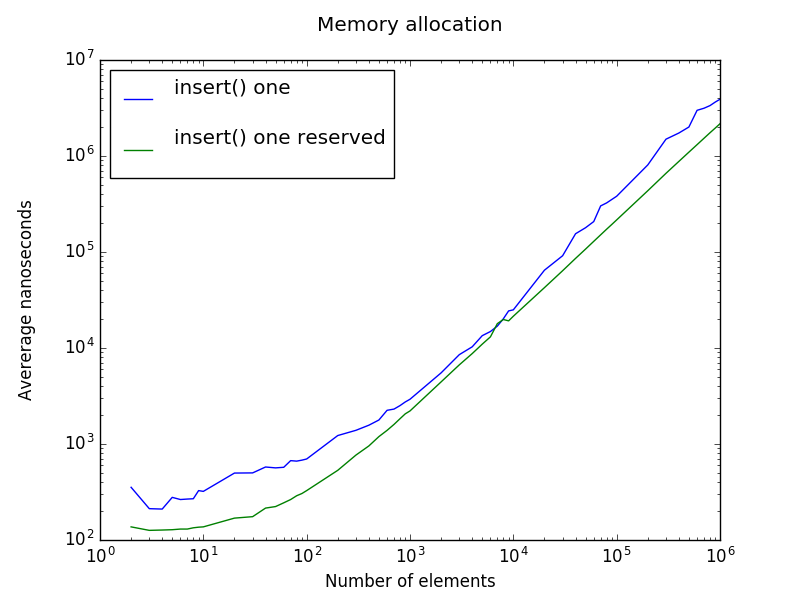
\includegraphics[width=.5\linewidth]{graphs/alloc_insert}
\end{center}
Here we see that calling \texttt{vector.reserve()} prior to the operations benefit the
performance.

Then, we have \texttt{vector.push\_back()}:
\begin{center}
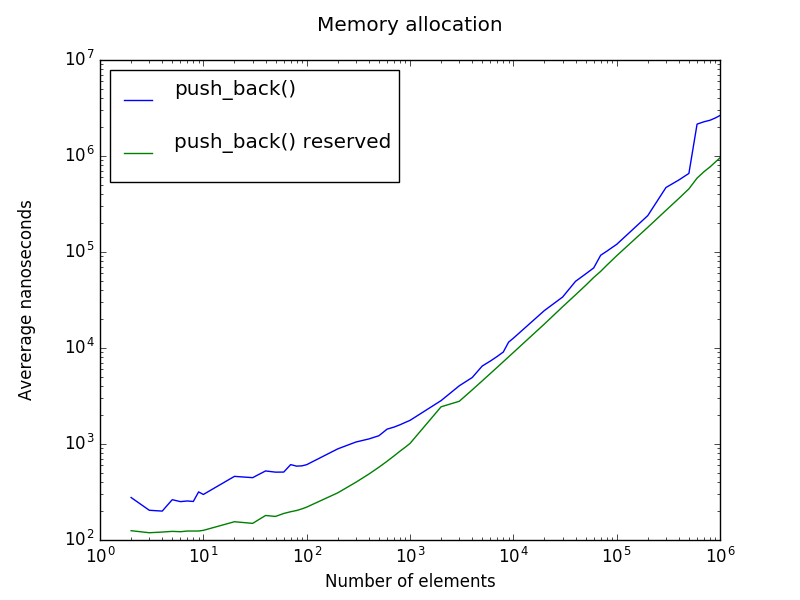
\includegraphics[width=.5\linewidth]{graphs/alloc_push}
\end{center}
Again, we see that calling \texttt{vector.reserve()} prior to the operations benefit the
performance.

To make sure, we have the graph containing both:
\begin{center}
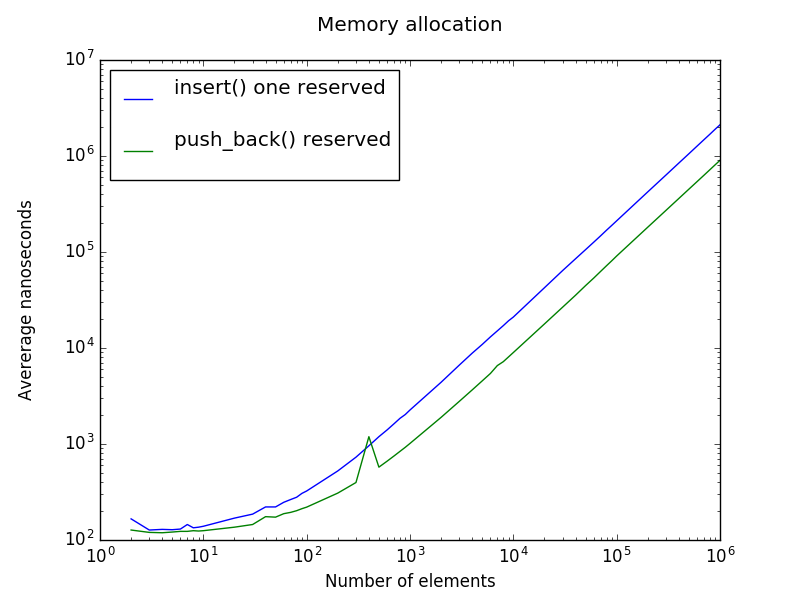
\includegraphics[width=.5\linewidth]{graphs/alloc_both}
\end{center}
From this graph, we see that calling \texttt{vector.push\_back()} gives the
best performance.

\subsubsection{Memory management and access}
When we want to move data from one \texttt{vector} to another, not empty,
\texttt{vector}. In these tests, we move a copy of a \texttt{vector} into the
original \texttt{vector}. We have following two approaches: manual move using
a for loop and using \texttt{vector.insert()}. For the manual move, we have
where we call \texttt{vector.size()} in the loop condition, and where we store
it in a variable before the loop. For insert, we have where we do and do not
call \texttt{vector.reserve()}.

Manual move:
\begin{center}
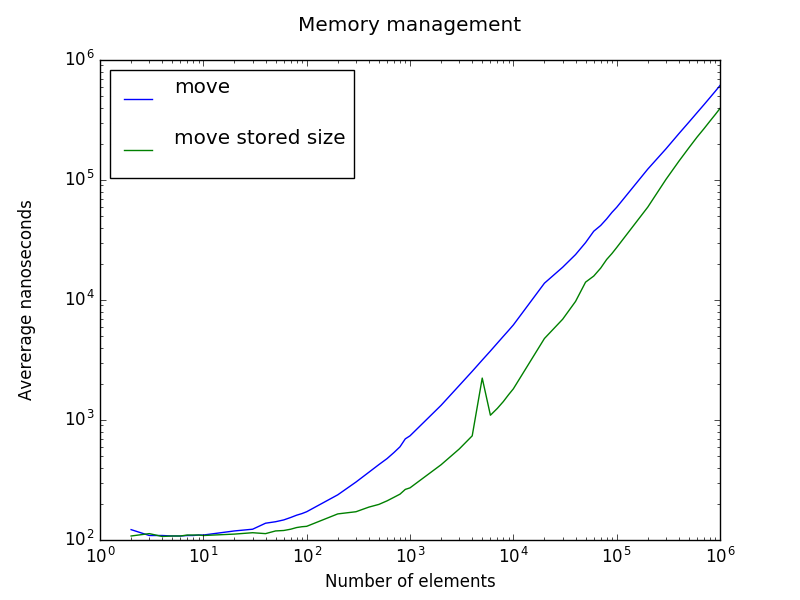
\includegraphics[width=.5\linewidth]{graphs/memman_move}
\end{center}
Here, we see that moving the call to \texttt{vector.size()} clearly improves
the performance.

\texttt{vector.insert()}:
\begin{center}
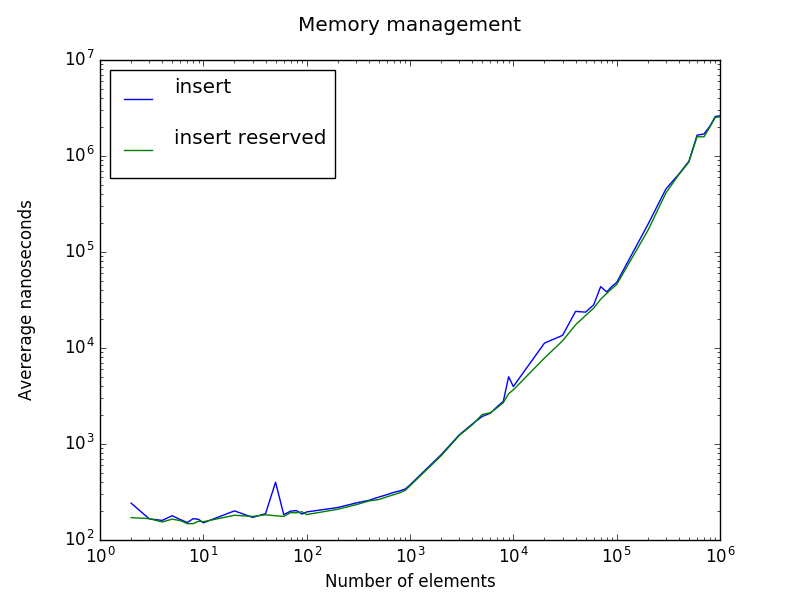
\includegraphics[width=.5\linewidth]{graphs/memman_insert}
\end{center}
strangely enough, even though we are moving a copy, calling
\texttt{vector.reserve()} beforehand improves performance.

Finally, we compare the two best:
\begin{center}
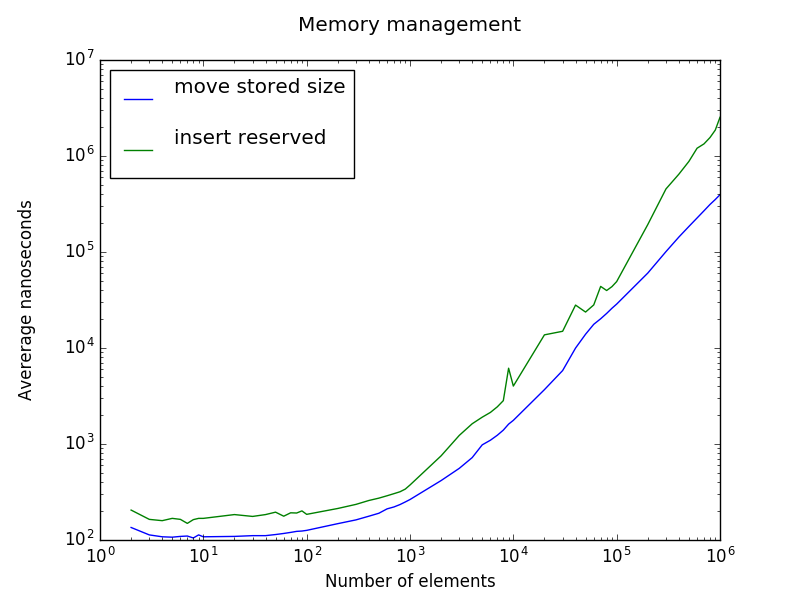
\includegraphics[width=.5\linewidth]{graphs/memman_both}
\end{center}
Here, we see that the manual move clearly beats the call to
\texttt{vector.insert()}

\subsubsection{Memory management into empty \texttt{vector}}
We have this test, to see the performance when copying a \texttt{vector} into
another empty \texttt{vector}. We have the following four approaches: using
\texttt{vecter.insert()}, using \texttt{vector.insert()} one element at a time,
using \texttt{vector.push\_back()} and using the constructor of \texttt{vector}.
Each of the first three are tested with and without using
\texttt{vector.reserve()} prior to the operations.

We start with \texttt{vector.insert()}:
\begin{center}
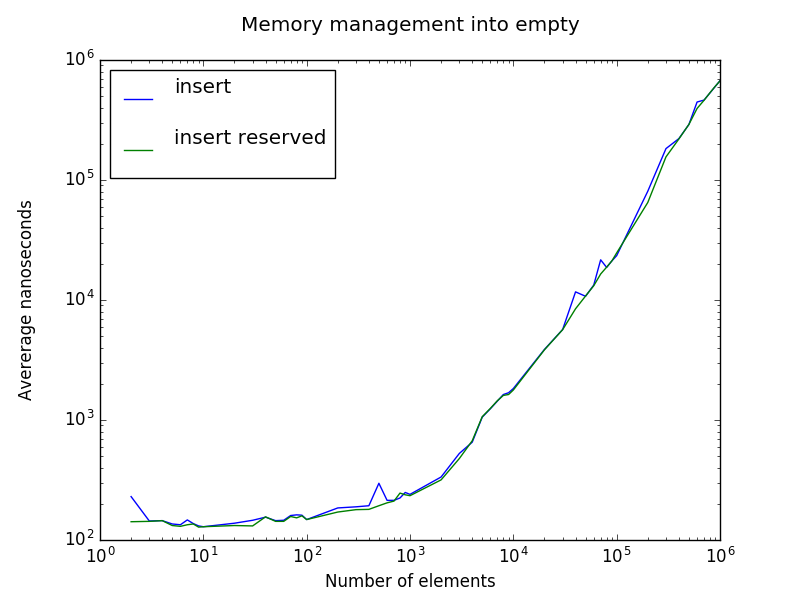
\includegraphics[width=.5\linewidth]{graphs/memmanempty_insert}
\end{center}

\texttt{vector.insert()} one element at the time:
\begin{center}
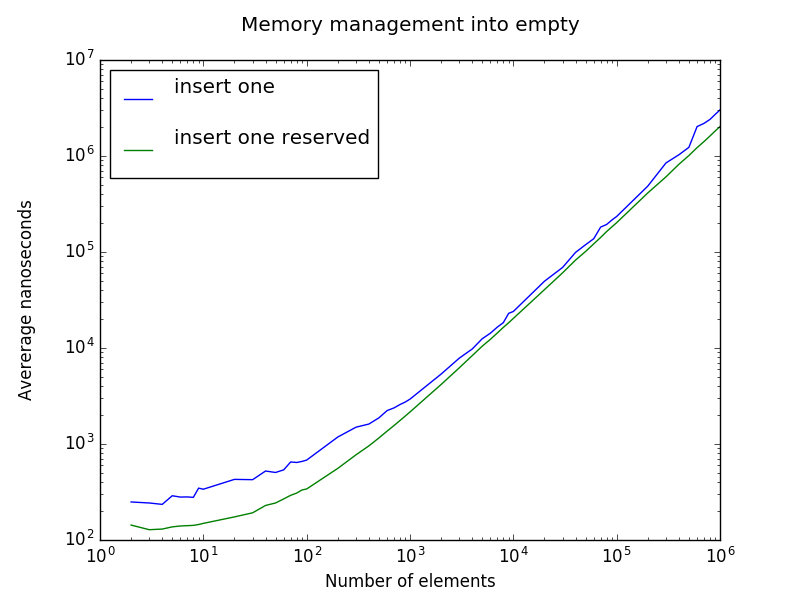
\includegraphics[width=.5\linewidth]{graphs/memmanempty_insertone}
\end{center}

\texttt{vector.push\_back()}:
\begin{center}
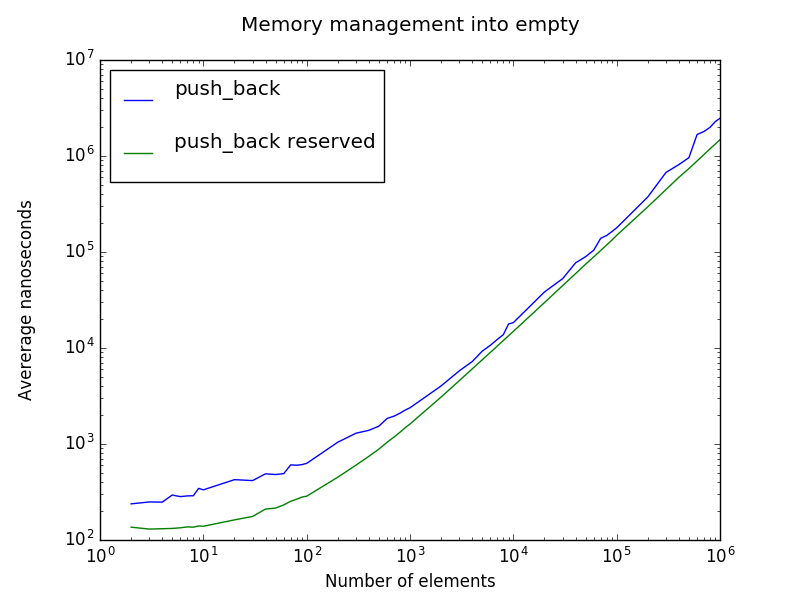
\includegraphics[width=.5\linewidth]{graphs/memmanempty_push}
\end{center}

Now, we see that the reserved \texttt{vector.insert()} has the highest
performance, so we will be using that for comparison to the constructor:
\begin{center}
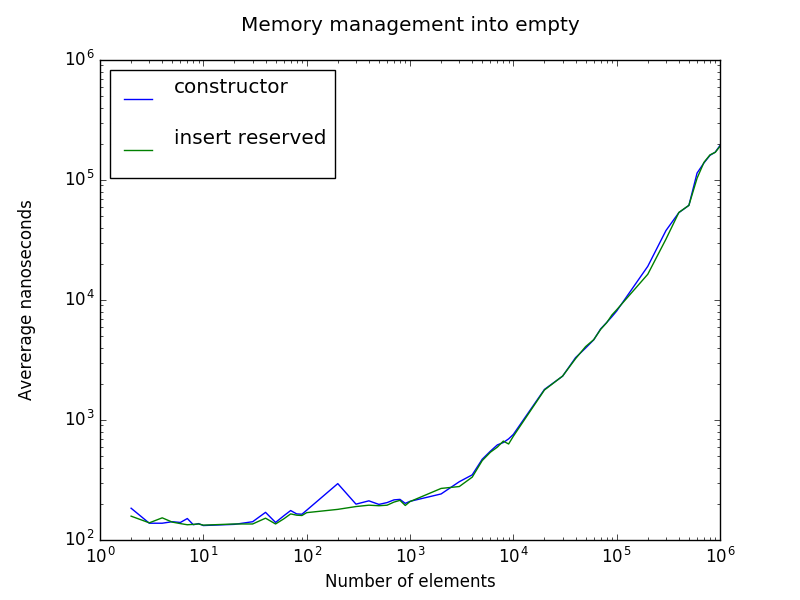
\includegraphics[width=.5\linewidth]{graphs/memmanempty_constr}
\end{center}
We see that in a few cases, calling \texttt{vector.insert()} beats using the
constructor. However, using the cunstructor makes the code simpler, in the
sense that it only uses 1 line of code, compared to the 3 lines of code when
using \texttt{vector.insert()}.

\subsection{Quicksort}
Quicksort is an algorithm, which is known to be good in practice. The
performance of the algorithm doues depend on the quality of the split, i.e. if
the splits are balanced. We have made different versions of Quicksort, and
modified them based on observations when running them.

\subsubsection{Sequential}
To start off, we implemented an in-place Quicksort, which we would then
parallize. To pick the pivot element, we just pick one at random.

\subsubsection{Naive parallel implementation}
The naive parallization, is to for each split, spawn a thread sorting each
split. This however, has a far too big overhead, which results in error on
larger input, as too many threads are spawned. On the smaller input, the
overhead from spawning threads is far greater than the gains from parallizing,
resulting in very bad performance, and as such we have not shown this approach
in our graphs.

\subsubsection{Limited parallel implementation}
Following the naive implementation, we tried to make the same approach, but
only spaw a limited number of threads. This did give a speedup, on larger
input. However, the performance of this approach depends a lot on the splits.
E.g. if we get a bad split in the beginning, i.e. one small portion and one big
portion, the thread getting the smaller portion finishes faster, and does not
do any work afterwards.

We also looked into if the bad performance could be due to the fact that the
threads share the memory. As such, we tried to instead of sending along a
pointer to the shared memory, we sent its own allocated \texttt{vector},
keeping the memory seperated. However, this made the performance worse. The
overhead introduced when moving memory into new memory is greater than the
gains. It does seem like since each thread works on its seperate part of the
shared memory, there are no problems. Furthermore, having seperate memory
doubles the memory used for every split, meaning we will have in the worst case
$O(n \ln n)$ memory usage instead of $O(n)$.

\subsubsection{Modified limited parallel implementation}
Following the idle threads from the previous implementation, we thought of
another way. We have a global integer variable, which denotes the maximum
number of threads. Each time a thread is spawned, the integer is decremented.
Every time a thread is done, the integer is incremented. As such, if a thread
is done with its part earlier than others, one of the threads with more work,
can spawn more threads, thus keeping the processor fed. However, there is a big
overhead, as the threads has to lock the variable when they are checking and
updating it. This results in a not optimal CPU utilisation.

\subsubsection{Thread pool approach}
Another approach to keeping the processor at work at all times, are a thread
pool approach. In this approach we have a queue and an array of threads. Each
thread tries to get a "job", which is two indices, indicating the start and the
end of the split to sort.

One problem we faced was when to stop the threads, as we could not use an empty
queue, as the queue starts empty, and there are no real way to know that the
entire input is sorted. The approach we took was to have a boolean value,
indicating whether or not the bottom has been reached. Once it has, and once
the queue is empty, threads return.

This approach keeps the processor at a high load. However, the overhead
introduced from creating, and synchronizing, i.e. mutex locking and unlocking,
is very large, so this approach only works on larger input, and even then it is
beaten by the limited parallel approach.

\subsection{Mergesort}
Mergesort is an algorithm, which is known to have very good performance when
having parallization. This is due to the equal splitting all the way through
the algorithm, which is always perfectly balanced. The hard part of this
algorithm was to make it in-place. We took a different approach: when we merge,
we copy one half of the input into a temporary vector, merge the temporary
vector and the other half into the original input.

\subsubsection{Sequential}
We started by making a normal sequential implementation. As this is
straightforward.

\subsubsection{Limited parallel}
We took the same initial approach to parallizing as in the limited parallel
Quicksort, i.e. spawing only a limited number of threads. Due to the balance of
Mergesort, the processor should be at work all the time. In practice this
worked very well.

We tried the same approach to seperate memory as with the parallel Quicksort.
Just as before, the overhead from managing memory outshines the gains from
having seperate memory.

\subsection{Combination of Quicksort and Mergesort}
As we can see in the sequential performance, Quicksort beats Mergesort.
However, when we look at the parallel performance, Mergesort beats Quicksort.
As such, we thought that a combination of the two would give the best
performance.

We start by using Mergesort on the top level, splitting the data in half, and
spawing a thread for each split. We keep doing this until we run out of
processor threads. When we do, we call the sequential Quicksort on the input,
as this should be faster when running sequential.

Compared to the other parallel implementations, our intuition worked, as soon
as the input gets large enough.



\section{Sorting networks}

\subsection{Testing}
Since it can be quite hard to see from the code if a specific sorting networks
should work, testing them is quite important. So for all the implemented
sorting networks for inputs $>4$ there is a test for a reserse sorted list, and
for a number of runs on random inputs. Futhermore there is the possibility to
run a full permutation test, that is testing the sorting networks for all
possible permutations of inputs of that size, though this should be possible to
make in $O(2^n)$ instead of the current $O(n!)$ due to the Zero-one principle.
This permutation test has been run on all the implemented sorting networks up
to and including \ttt{nsort\_13()}


\section{Ford Johnson}
When considering element comparison in sorting smaller sets of numbers the algorithm by Ford \& Johnson is a classical example\cite{fj59}. It is close to optimal in the number of element comparisons it needs to sort smaller sets of numbers \cite{m77}. We have implemented an in-place version of the Ford Johnson algorithm following the outline by Ford \& Johnson\cite{fj59}.

\subsection{Branch optimization}
The Ford \& Johnson may be close to optimal in number of element comparisons made, but it relies on binary search among other sub procedures. These along with the main method uses branching to choose between two ways through the code. This will make it difficult for the compiler to pipeline the instructions in a way that optimizes the runtime, due to the potential flushes of misspredicting the branches.

Motivated by this we have further implemented a version of Ford \& Johnson where the branches has been optimized out. This has generally been done by utilizing the boolean values in the mathematical statements, used throughout the code, in order to capture the branching in statements that can be better anticipated by the compiler.
\begin{figure}
	\caption{Comparison of small sets specialized sortes and std::sort}
	\label{smalltablefigure}
	\begin{tabular}{|l|l|l|l|l|}\hline
	size&std::sort&Sorting networks&Ford Johnson&fj branch optimized\\\hline
	2&293&287&647&646\\
	4&567&277&1079&1142\\
	6&350&348&1984&2014\\
	8&404&418&2371&2409\\
	10&445&521&3482&3386\\
	12&473&538&3664&3807\\
	14&520&608&5176&5341\\
	16&611&685&5832&5792\\\hline
\end{tabular}
\end{figure}

\bibliographystyle{DIKU} % Use DIKU-alternative for the other citation style
\bibliography{bib}

\newpage
\appendix
This is a compilation of figures of the sorting networks implemented.
\begin{figure}[htb]
 \centering
    \begin{subfigure}[b]{0.3\textwidth}
        \centering
        \begin{sortingnetwork}{3}{0.4}
            \nodeconnection{ {2,3}}
            \addtocounter{sncolumncounter}{2}
            \nodeconnection{ {1,2}}
            \addtocounter{sncolumncounter}{2}
            \nodeconnection{ {2,3}}
        \end{sortingnetwork}
        \subcaption{3-input}
    \end{subfigure}
    \begin{subfigure}[b]{0.3\textwidth}
        \centering
        \begin{sortingnetwork}{4}{0.4}
            \nodeconnection{ {1,2}, {3,4}}
            \addtocounter{sncolumncounter}{2}
            \nodeconnection{ {1,3}}
            \nodeconnection{ {2,4}}
            \addtocounter{sncolumncounter}{2}
            \nodeconnection{ {2,3}}
        \end{sortingnetwork}
        \subcaption{4-input}
    \end{subfigure}
    \begin{subfigure}[b]{0.33\textwidth}
        \centering
        \begin{sortingnetwork}{5}{0.4}
            \nodeconnection{ {2,3}, {4,5}}
            \addtocounter{sncolumncounter}{2}
            \nodeconnection{ {1,3}}
            \nodeconnection{ {2,4}}
            \addtocounter{sncolumncounter}{2}
            \nodeconnection{ {3,5}}
            \nodeconnection{ {1,4}}
            \addtocounter{sncolumncounter}{2}
            \nodeconnection{ {1,2}}
            \nodeconnection{ {3,4}}
            \addtocounter{sncolumncounter}{2}
            \nodeconnection{ {2,3}}
        \end{sortingnetwork}
        \subcaption{5-input}
    \end{subfigure}
 \caption{3-5 input length optimal sorting networks \cite{ron-zeno}}
 \label{fig:sort-5}
\end{figure}


\begin{figure}[htb]
 \centering
    \begin{subfigure}[b]{0.45\textwidth}
        \centering
        \begin{sortingnetwork}{6}{0.4}
            \nodeconnection{ {1,2}, {3,4}, {5,6}}
            \addtocounter{sncolumncounter}{2}
            \nodeconnection{ {1,3}, {4,6}}
            \nodeconnection{ {2,5}}
            \addtocounter{sncolumncounter}{2}
            \nodeconnection{ {1,2}, {3,4}, {5,6}}
            \addtocounter{sncolumncounter}{2}
            \nodeconnection{ {2,3}, {4,5}}
            \addtocounter{sncolumncounter}{2}
            \nodeconnection{ {3,4}}
        \end{sortingnetwork}
        \subcaption{6-input}
    \end{subfigure}
    \begin{subfigure}[b]{0.45\textwidth}
        \centering
        \begin{sortingnetwork}{7}{0.4}
            \nodeconnection{ {2,3}, {4,5}, {6,7}}
            \addtocounter{sncolumncounter}{2}
            \nodeconnection{ {1,3}, {5,7}}
            \nodeconnection{ {4,6}}
            \addtocounter{sncolumncounter}{2}
            \nodeconnection{ {3,7}}
            \nodeconnection{ {2,6}}
            \nodeconnection{ {1,5}}
            \addtocounter{sncolumncounter}{2}
            \nodeconnection{ {3,6}}
            \nodeconnection{ {1,4}}
            \addtocounter{sncolumncounter}{2}
            \nodeconnection{ {3,5}}
            \nodeconnection{ {2,4}}
            \addtocounter{sncolumncounter}{2}
            \nodeconnection{ {1,2}, {3,4}, {5,6}}
        \end{sortingnetwork}
        \subcaption{7-input}
    \end{subfigure}
 \caption{6 and 7 input length optimal sorting networks \cite{ron-zeno}}
 \label{fig:sort-7}
\end{figure}


\begin{figure}[htb]
 \centering
    \begin{subfigure}[b]{0.45\textwidth}
        \centering
        \begin{sortingnetwork}{8}{0.4}
            \nodeconnection{{1,8}}
            \nodeconnection{{2,7}}
            \nodeconnection{{3,6}}
            \nodeconnection{{4,5}}
            \addtocounter{sncolumncounter}{2}
            \nodeconnection{ {1,4}, {5,8}}
            \nodeconnection{ {2,3}, {6,7}}
            \addtocounter{sncolumncounter}{2}
            \nodeconnection{ {1,2}, {3,4}, {5,6}, {7,8}}
            \addtocounter{sncolumncounter}{2}
            \nodeconnection{ {4,6}, {3,5}}
            \addtocounter{sncolumncounter}{2}
            \nodeconnection{ {2,3}, {4,5}, {6,7}}
            \nodeconnection{ {3,4}, {5,6}}
        \end{sortingnetwork}
        \subcaption{8-input}
    \end{subfigure}
    \begin{subfigure}[b]{0.5\textwidth}
        \centering
        \begin{sortingnetwork}{9}{0.4}
            \nodeconnection{ {2,9}}
            \nodeconnection{ {3,8}}
            \nodeconnection{ {4,7}}
            \nodeconnection{ {5,6}}
            \addtocounter{sncolumncounter}{2}
            \nodeconnection{ {2,5}, {6,9}}
            \nodeconnection{ {1,3}, {7,8}}
            \addtocounter{sncolumncounter}{2}
            \nodeconnection{ {3,7}, {8,9}}
            \nodeconnection{ {1,4}, {5,6}}
            \addtocounter{sncolumncounter}{2}
            \nodeconnection{ {1,2}, {4,6}, {7,8}}
            \nodeconnection{ {3,5}}
            \addtocounter{sncolumncounter}{2}
            \nodeconnection{ {2,4}, {6,8}}
            \nodeconnection{ {5,7}}
            \addtocounter{sncolumncounter}{2}
            \nodeconnection{ {2,3}, {4,5}, {6,7}, {8,9}}
            \addtocounter{sncolumncounter}{2}
            \nodeconnection{ {3,4}, {5,6}}
        \end{sortingnetwork}
        \subcaption{9-input}
    \end{subfigure}
 \caption{8 and 9 input length optimal sorting networks \cite{ron-zeno}}
 \label{fig:sort-9}
\end{figure}


\begin{figure}[htb]
 \centering
    \begin{subfigure}[b]{0.45\textwidth}
        \centering
        \begin{sortingnetwork}{10}{0.4}
            \nodeconnection{{1,2}, {3,4}, {5,6}, {7,8}, {9,10}}
            \addtocounter{sncolumncounter}{2}
            \nodeconnection{ {5,10}}
            \nodeconnection{ {1,6}}
            \nodeconnection{ {2,9}}
            \nodeconnection{ {4,8}}
            \nodeconnection{ {3,7}}
            \addtocounter{sncolumncounter}{2}
            \nodeconnection{ {1,3}, {4,7}, {8,10}}
            \nodeconnection{ {2,5}, {6,9}}
            \addtocounter{sncolumncounter}{2}
            \nodeconnection{ {1,2}, {3,8}, {9,10}}
            \nodeconnection{ {5,7}}
            \nodeconnection{ {4,6}}
            \addtocounter{sncolumncounter}{2}
            \nodeconnection{ {3,5}, {7,9}}
            \nodeconnection{ {2,4}, {6,8}}
            \addtocounter{sncolumncounter}{2}
            \nodeconnection{ {2,3}, {4,5}, {6,7}, {8,9}}
            \addtocounter{sncolumncounter}{2}
            \nodeconnection{ {3,4}, {5,6}, {7,8}}
        \end{sortingnetwork}
        \subcaption{10-input}
    \end{subfigure}
    \begin{subfigure}[b]{0.6\textwidth}
        \centering
        \begin{sortingnetwork}{11}{0.4}
            \nodeconnection{ {1,10}}
            \nodeconnection{ {2,9}}
            \nodeconnection{ {3,8}}
            \nodeconnection{ {4,7}}
            \nodeconnection{ {5,6}}
            \addtocounter{sncolumncounter}{2}
            \nodeconnection{ {1,4}, {5,11}}
            \nodeconnection{ {2,3}, {7,10}}
            \nodeconnection{ {8,9}}
            \addtocounter{sncolumncounter}{2}
            \nodeconnection{ {1,2}, {3,4}, {6,9}, {10,11}}
            \nodeconnection{ {7,8}}
            \addtocounter{sncolumncounter}{2}
            \nodeconnection{ {2,3}, {4,6}, {9,11}}
            \nodeconnection{ {5,10}}
            \addtocounter{sncolumncounter}{2}
            \nodeconnection{ {1,5}, {8,9}}
            \nodeconnection{ {2,6}}
            \nodeconnection{ {3,10}}
            \nodeconnection{ {4,7}}
            \addtocounter{sncolumncounter}{2}
            \nodeconnection{ {2,5}, {6,8}}
            \nodeconnection{ {3,4}, {7,10}}
            \addtocounter{sncolumncounter}{2}
            \nodeconnection{ {3,5}, {7,8}, {9,10}}
            \nodeconnection{ {4,6}}
            \addtocounter{sncolumncounter}{2}
            \nodeconnection{ {4,5}, {6,7}, {8,9}}
        \end{sortingnetwork}
        \subcaption{11-input}
    \end{subfigure}
 \caption{10 input length optimal, and 11 input best known sorting networks
 \cite{ron-zeno}}

 \label{fig:sort-11}
\end{figure}

\begin{figure}[htb]
 \centering
    \centering
    \begin{sortingnetwork}{12}{0.4}
        \nodeconnection{ {1,10}}
        \nodeconnection{ {2,9}}
        \nodeconnection{ {3,8}}
        \nodeconnection{ {4,7}}
        \nodeconnection{ {5,6}}
        \addtocounter{sncolumncounter}{2}
        \nodeconnection{ {1,4}, {5,11}}
        \nodeconnection{ {2,3}, {7,10}}
        \nodeconnection{ {8,9}}
        \addtocounter{sncolumncounter}{2}
        \nodeconnection{ {1,2}, {3,4}, {6,9}, {10,11}}
        \nodeconnection{ {7,8}}
        \addtocounter{sncolumncounter}{2}
        \nodeconnection{ {2,3}, {4,6}, {9,11}}
        \nodeconnection{ {5,10}}
        \addtocounter{sncolumncounter}{2}
        \nodeconnection{ {1,5}, {8,9}}
        \nodeconnection{ {2,6}}
        \nodeconnection{ {3,10}}
        \nodeconnection{ {4,7}}
        \addtocounter{sncolumncounter}{2}
        \nodeconnection{ {2,5}, {6,8}}
        \nodeconnection{ {3,4}, {7,10}}
        \addtocounter{sncolumncounter}{2}
        \nodeconnection{ {3,5}, {7,8}, {9,10}}
        \nodeconnection{ {4,6}}
        \addtocounter{sncolumncounter}{2}
        \nodeconnection{ {4,5}, {6,7}, {8,9}}
    \end{sortingnetwork}
 \caption{12 input best known sorting networks \cite{ron-zeno}}
 \label{fig:sort-12}
\end{figure}


\begin{figure}[htb]
 \centering
    \centering
    \begin{sortingnetwork}{13}{0.4}
        \nodeconnection{ {1,2}, {3,4}, {5,6}, {7,8}, {9,10}, {11,12}}
        \addtocounter{sncolumncounter}{2}
        \nodeconnection{ {2,4}, {6,8}, {10,12}}
        \nodeconnection{ {1,3}, {5,7}, {9,11}}
        \addtocounter{sncolumncounter}{2}
        \nodeconnection{ {4,8}}
        \nodeconnection{ {3,7}}
        \nodeconnection{ {2,6}}
        \nodeconnection{ {1,5}, {9,13}}
        \addtocounter{sncolumncounter}{2}
        \nodeconnection{ {5,13}}
        \nodeconnection{ {4,12}}
        \nodeconnection{ {3,11}}
        \nodeconnection{ {2,10}}
        \nodeconnection{ {1,9}}
        \addtocounter{sncolumncounter}{2}
        \nodeconnection{ {6,11}}
        \nodeconnection{ {7,10}}
        \nodeconnection{ {2,3}, {4,13}}
        \nodeconnection{ {5,9}}
        \nodeconnection{ {8,12}}
        \addtocounter{sncolumncounter}{2}
        \nodeconnection{ {3,9}}
        \nodeconnection{ {2,5}}
        \addtocounter{sncolumncounter}{2}
        \nodeconnection{ {3,5}, {6,7}, {10,11}}
        \nodeconnection{ {8,13}}
        \nodeconnection{ {4,9}}
        \addtocounter{sncolumncounter}{2}
        \nodeconnection{ {4,6}, {8,10}}
        \nodeconnection{ {7,9}, {11,13}}
        \addtocounter{sncolumncounter}{2}
        \nodeconnection{ {4,5}, {6,7}, {8,9}, {10,11}, {12,13}}
        \nodeconnection{ {7,8}, {9,10}}
    \end{sortingnetwork}
 \caption{13 input sorting network, derived from Greens 16 input sorting
    network \cite{hugues-juille}}
 \label{fig:sort-13}
\end{figure}

\begin{figure}[htb]
 \centering
    \centering
    \begin{sortingnetwork}{14}{0.4}
        \nodeconnection{ {1,2}, {3,4}, {5,6}, {7,8}, {9,10}, {11,12}, {13,14}}
        \addtocounter{sncolumncounter}{2}
        \nodeconnection{ {2,4}, {6,8}, {10,12}}
        \nodeconnection{ {1,3}, {5,7}, {9,11}}
        \addtocounter{sncolumncounter}{2}
        \nodeconnection{ {4,8}}
        \nodeconnection{ {3,7}}
        \nodeconnection{ {2,6}, {10,14}}
        \nodeconnection{ {1,5}, {9,13}}
        \addtocounter{sncolumncounter}{2}
        \nodeconnection{ {6,14}}
        \nodeconnection{ {5,13}}
        \nodeconnection{ {4,12}}
        \nodeconnection{ {3,11}}
        \nodeconnection{ {2,10}}
        \nodeconnection{ {1,9}}
        \addtocounter{sncolumncounter}{2}
        \nodeconnection{ {6,11}}
        \nodeconnection{ {7,10}}
        \nodeconnection{ {2,3}, {4,13}}
        \nodeconnection{ {5,9}}
        \nodeconnection{ {8,12}}
        \addtocounter{sncolumncounter}{2}
        \nodeconnection{ {3,9}}
        \nodeconnection{ {2,5}, {8,14}}
        \addtocounter{sncolumncounter}{2}
        \nodeconnection{ {3,5}, {6,7}, {10,11}, {12,14}}
        \nodeconnection{ {8,13}}
        \nodeconnection{ {4,9}}
        \addtocounter{sncolumncounter}{2}
        \nodeconnection{ {4,6}, {8,10}}
        \nodeconnection{ {7,9}, {11,13}}
        \addtocounter{sncolumncounter}{2}
        \nodeconnection{ {4,5}, {6,7}, {8,9}, {10,11}, {12,13}}
        \nodeconnection{ {7,8}, {9,10}}
    \end{sortingnetwork}
 \caption{14 input sorting network, derived from Greens 16 input sorting
    network \cite{hugues-juille}}
 \label{fig:sort-14}
\end{figure}


\begin{figure}[htb]
 \centering
    \centering
    \begin{sortingnetwork}{15}{0.4}
        \nodeconnection{ {1,2}, {3,4}, {5,6}, {7,8}, {9,10}, {11,12}, {13,14}}
        \addtocounter{sncolumncounter}{2}
        \nodeconnection{ {2,4}, {6,8}, {10,12}}
        \nodeconnection{ {1,3}, {5,7}, {9,11}, {13,15}}
        \addtocounter{sncolumncounter}{2}
        \nodeconnection{ {4,8}}
        \nodeconnection{ {3,7}, {11,15}}
        \nodeconnection{ {2,6}, {10,14}}
        \nodeconnection{ {1,5}, {9,13}}
        \addtocounter{sncolumncounter}{2}
        \nodeconnection{ {7,15}}
        \nodeconnection{ {6,14}}
        \nodeconnection{ {5,13}}
        \nodeconnection{ {4,12}}
        \nodeconnection{ {3,11}}
        \nodeconnection{ {2,10}}
        \nodeconnection{ {1,9}}
        \addtocounter{sncolumncounter}{2}
        \nodeconnection{ {6,11}}
        \nodeconnection{ {7,10}}
        \nodeconnection{ {2,3}, {4,13}}
        \nodeconnection{ {5,9}}
        \nodeconnection{ {8,12}, {14,15}}
        \addtocounter{sncolumncounter}{2}
        \nodeconnection{ {3,9}, {12,15}}
        \nodeconnection{ {2,5}, {8,14}}
        \addtocounter{sncolumncounter}{2}
        \nodeconnection{ {3,5}, {6,7}, {10,11}, {12,14}}
        \nodeconnection{ {8,13}}
        \nodeconnection{ {4,9}}
        \addtocounter{sncolumncounter}{2}
        \nodeconnection{ {4,6}, {8,10}}
        \nodeconnection{ {7,9}, {11,13}}
        \addtocounter{sncolumncounter}{2}
        \nodeconnection{ {4,5}, {6,7}, {8,9}, {10,11}, {12,13}}
        \nodeconnection{ {7,8}, {9,10}}
    \end{sortingnetwork}
 \caption{15 input sorting network, derived from Greens 16 input sorting
    network \cite{hugues-juille}}
 \label{fig:sort-15}
\end{figure}

\begin{figure}[htb]
 \centering
    \centering
    \begin{sortingnetwork}{16}{0.4}
        \nodeconnection{ {1,2}, {3,4}, {5,6}, {7,8}, {9,10}, {11,12}, {13,14},
        {15,16}}
        \addtocounter{sncolumncounter}{2}
        \nodeconnection{ {2,4}, {6,8}, {10,12}, {14,16}}
        \nodeconnection{ {1,3}, {5,7}, {9,11}, {13,15}}
        \addtocounter{sncolumncounter}{2}
        \nodeconnection{ {4,8}, {12,16}}
        \nodeconnection{ {3,7}, {11,15}}
        \nodeconnection{ {2,6}, {10,14}}
        \nodeconnection{ {1,5}, {9,13}}
        \addtocounter{sncolumncounter}{2}
        \nodeconnection{ {8,16}}
        \nodeconnection{ {7,15}}
        \nodeconnection{ {6,14}}
        \nodeconnection{ {5,13}}
        \nodeconnection{ {4,12}}
        \nodeconnection{ {3,11}}
        \nodeconnection{ {2,10}}
        \nodeconnection{ {1,9}}
        \addtocounter{sncolumncounter}{2}
        \nodeconnection{ {6,11}}
        \nodeconnection{ {7,10}}
        \nodeconnection{ {2,3}, {4,13}}
        \nodeconnection{ {5,9}}
        \nodeconnection{ {8,12}, {14,15}}
        \addtocounter{sncolumncounter}{2}
        \nodeconnection{ {3,9}, {12,15}}
        \nodeconnection{ {2,5}, {8,14}}
        \addtocounter{sncolumncounter}{2}
        \nodeconnection{ {3,5}, {6,7}, {10,11}, {12,14}}
        \nodeconnection{ {8,13}}
        \nodeconnection{ {4,9}}
        \addtocounter{sncolumncounter}{2}
        \nodeconnection{ {4,6}, {8,10}}
        \nodeconnection{ {7,9}, {11,13}}
        \addtocounter{sncolumncounter}{2}
        \nodeconnection{ {4,5}, {6,7}, {8,9}, {10,11}, {12,13}}
        \nodeconnection{ {7,8}, {9,10}}
    \end{sortingnetwork}
 \caption{Greens 16 input sorting networks \cite{hugues-juille}}
 \label{fig:sort-16}
\end{figure}



\end{document}
